\documentclass{article}
\usepackage{graphicx} % Required for inserting images
\usepackage{mdframed}
\usepackage{amsmath, yhmath}
\usepackage{amssymb}
\usepackage[textheight = 24cm]{geometry} 
\usepackage[font = sf, justification=raggedright]{caption} 
\usepackage{array}
\usepackage{hhline} 
\usepackage{pgfplots}
\pgfplotsset{compat=1.15}
\usepackage{mathrsfs}
\usepackage[most]{tcolorbox}
\usetikzlibrary{calc}
\usepackage[math]{cellspace}
\usepackage{tikz}
%\usepackage{darkmode} \enabledarkmode
\usetikzlibrary{intersections}
\usetikzlibrary[arrows.meta]
\cellspacetoplimit 4pt
\cellspacebottomlimit 4pt

% Commands new
\tcbuselibrary{skins, breakable}
\tcbset{
	myboxstyle/.style={
		breakable,
		colback=white,            % Background color for the content
		colframe=black,           % Frame color
		colbacktitle=gray!15,     % Background color for the title
		coltitle=black,           % Text color for the title
		fonttitle=\bfseries,      %
		title={#1},               % The title content will be passed as an argument
		enhanced,
		attach boxed title to top left={yshift=-2mm, xshift=2mm},
		boxed title style={
			colframe=black,
			arc=1mm,
			outer arc=1.5mm,
			boxrule=0.5mm,        % Border thickness for the title
		},
		overlay={},
	}
}

% Define the 'exercise' environment to use the custom style

\newenvironment{exercise} {
	\begin{tcolorbox}[myboxstyle={Problem 1}]
	}{
	\end{tcolorbox}
}

\newmdtheoremenv{theo}{Theorem}
\newcommand{\ej}{\hspace{0.5cm}ej\hspace{0.5cm}}


\title{Nahuel Notes}
\author{Alejandro Ceccheto}
\date{February 2024}


%% Notes
% La = intervalo semi abierto por izquierda.
% Lb = intervalo semi abierto por derecha.
% Lc = intervalo abierto hasta el infinito.
% Lq = intervalo abierto.
% Ld = intervalo cerrado.

\begin{document}
	
	\maketitle
	
	
	\pagebreak
	\tableofcontents
	\pagebreak
	
	
	\section{Números Reales y sus operaciones}
	\begin{theo}
		Los números reales comprende todos los números que pueden llegar a aparecer dentro de una recta real $\mathbb{R}$, sean enteros $\mathbb{Z}$, naturales $\mathbb{N}$, racionales $\mathbb{Q}$ e irracionales $\mathbb{I}$
	\end{theo}
	
	\vspace{1cm}
	
	Example : \\ 
	
	$\mathbb{N} = 1, 2, 3, \dots$ \\
	
	$\mathbb{Q} = \frac{1}{2}, 0.4, \dots$ \\
	
	$\mathbb{I} = \sqrt{2}, \sqrt{7}, \pi, e, \dots$ \\
	
	$\mathbb{Z} = -536, -345, -1, -2, \dots$ \\
	
	En resumen, los numeros $\mathbb{R}$ comprendes todos los numeros que existen siempre y cuando no nos metamos en los numero complejos $\mathbb{C}$.
	
	
	\subsection{Reglas de Fracciones}
	
\begin{itemize}
	\item{Suma de Fracciones}
	\begin{equation*}
		\frac{a}{b} + \frac{c}{d} = \frac{ad+bc}{bd} \hspace{0.5cm} Ej: \frac{4}{5} + \frac{5}{3} = \frac{4*3 + 5*5}{5*3} = \frac{37}{15} = 2,4\wideparen{6}
	\end{equation*}
	\item{Resta de fracciones}
	\begin{equation*}
		\frac{a}{b} - \frac{d}{c} = \frac{ad-bc}{bd} \hspace{0.5cm} Ej: \frac{2}{3} - \frac{3}{4}  \rightarrow \frac{2*4 + 3*3}{3*4} = \frac{8-9}{12}= \frac{-1}{12}
	\end{equation*}
	\item{multiplicación de fracciones}
	\begin{equation*}
		\frac{a}{b} \cdot \frac{c}{d} = \frac{ac}{bd} \hspace{0.5cm}ej\hspace{0.5cm} \frac{1}{2} \cdot \frac{2}{1} = \frac{2}{2}
	\end{equation*}
	\item{División de fracciones}
	\begin{equation*}
		\frac{a}{b} \div \frac{c}{d} = \frac{a}{b} \cdot \frac{d}{c} = \frac{a \cdot d}{b \cdot c} \hspace{0.5cm}ej\hspace{0.5cm} \frac{5}{7} \div \frac{1}{6} = \frac{5}{7} \cdot \frac{6}{1} = \frac{30}{1}
	\end{equation*}
\end{itemize}
	\pagebreak
	\subsection{Pasar de Fracción a mixto o decimal y vice-versa}
		\begin{theo}
			Para pasar un numero de Fracción a decimal, lo único que tenemos que hacer dividir los números dados en la fracción, pero de decimal, mixto o periódico a fracción es algo mas complicado.
		\end{theo} 
		
		Ejemplos de como se hace : \\
	\begin{center}
		
			De fracción a decimal
	\end{center}
	\begin{equation*}
		\frac{1}{2} = 0.5
	\end{equation*}
	\begin{center}
		De decimal a fracción (siendo este un numero ni peridico ni mixto lo que se hace es poner ceros tantos numeros haya atras del punto)
	\end{center}
	\begin{equation*}
		0.5 = \frac{5}{10} = \frac{1}{2}
	\end{equation*}
	\begin{center}
		de decimal periódico a fracción (en este caso, tenemos un numero periódico, por lo tanto se re escribe el numerador (parte de arriba), como la resta entre todo el numero sin coma, menos la parte entera, y luego siempre que tengamos un numero periódico, en el denominador va tantos 9 como numeros periodicos haya).
	\end{center}
	
	\begin{equation*}
		2.\wideparen{5} = \frac{25 - 2}{9} = \frac{23}{9}
	\end{equation*}
	\begin{center}
		Para convertir un numero periódico mixto a fracción es también algo mas complicado, requiere saber las propiedades anteriores, por ejemplo, supongamos que quiero convertir $3.12\wideparen{3}$ a fracción, esto es lo que se tiene que hacer.
	\end{center}
	 \begin{equation*}
	 	3.12\wideparen{3} = \frac{3123-312}{900} = \frac{2811}{900} = \frac{937}{300}
	 \end{equation*}
	 
	Acá lo que se hizo fue simplemente lo mismo de arriba, que por cada numero que este atrás de la coma y no sea periódico, se agregaron 0, pero por cada numero que si fue periódico, se agrega un 9. y el resto se resuelve tal como esta.
	
	\pagebreak
	\subsection{Reglas de Exponentes}
	\begin{theo}
		En pocas palabras, Exponentes hace referencia a la elevación de un numero a otro $x^n$ y radicales hace referencia a la raíz de un numero $\sqrt{x}$
	\end{theo}
	\hspace{1cm}
	con esto en mente, los exponentes y radicales llevan de por si propiedades que se deberían saber para operar con ellos cada ves que se presente un ejercicio
	
	

\begin{itemize}
	
	
	\item{potencia de 0 = 0}
	\begin{equation*}
		a^0 = 0  \hspace{0.5cm}ej\hspace{0.5cm} 2^0 = 0
	\end{equation*}
	\item{Potencia de 1 = n}
	\begin{equation*}
		a^1 = a \hspace{0.5cm}ej\hspace{0.5cm} 2^1 = 2
	\end{equation*}
	\item{Potencia de exponente entero negativo $a^{-1}$}
	\begin{equation*}
		a^{-n} = \frac{1}{a^n} \hspace{0.5cm}ej\hspace{0.5cm} 3^{-2} = \frac{1}{3^2} = \frac{1}{6} \hspace{1cm} a \neq 0
	\end{equation*}
	\item{Potencia de exponente racional}
	\begin{equation*}
		a^{\frac{m}{n}} = \sqrt[n]{a^m} \hspace{0.5cm}ej\hspace{0.5cm} 2{\frac{1}{2}} = \sqrt{2} 
	\end{equation*}
	
	\item{Potencia de exponente racional y negativo}
	\begin{equation*}
		a^{-\frac{m}{n}} = \frac{1}{\sqrt[n]{a^m}} \hspace{0.5cm}ej\hspace{0.5cm} 2^{-\frac{1}{2}} = \frac{1}{\sqrt[n]{a^m}}
	\end{equation*}
	
	\item{Multiplicación de potencias con la misma base}
	\begin{equation*}
		a^n\cdot a^m = a^{n+m} \hspace{0.5cm}ej\hspace{0.5cm} 2^2 \cdot 2^3 = 2^{2+3} = 2^5 = 32
	\end{equation*}
	
	
	\item{División de potencias con la misma base}
	\begin{equation*}
		\frac{a^n}{a^m} = a^{n-m} \hspace{0.5cm}ej\hspace{0.5cm} \frac{2^2}{2^5} = 2^{2-5} = 2^{-3} = \frac{1}{2^3} = \frac{1}{6} 
	\end{equation*}
	
	\item{Potencia de una Potencia}
	\begin{equation*}
		{a^n}^m = a^{n+m} \hspace{0.5cm}ej\hspace{0.5cm} {2^2}^2 = 2^{2+2} = 2^4 = 16
	\end{equation*}
	\item{Producto de potencia con el mismo exponente}
	\begin{equation*}
		a^n\cdot b^n = (a\cdot b)^n \hspace{0.5cm}ej\hspace{0.5cm} 2^2 \cdot 3^2 = (2 \cdot 3)^2
	\end{equation*}
	\item{Cociente de potencias con el mismo exponente}
	\begin{equation*}
		\frac{a^n}{b^n} = \left(\frac{a}{b} \right)^n \hspace{0.5cm}ej\hspace{0.5cm} \frac{-6^3}{2^3} = \left( \frac{-6}{2} \right)^3 = (-3)^3 = -27
	\end{equation*}
\end{itemize}
	 \pagebreak

	\subsection{Reglas de radicales}
	\begin{itemize}
		\item{ley de cancelación de radical}
		
		Una raiz n elevada a la potencia n se cancela
		\begin{equation*}
			\sqrt[n]{a}^n = a  \hspace{0.5cm}ej\hspace{0.5cm} \sqrt{6}^2 = 6
		\end{equation*}
		
		
		\item{Raiz de una multiplicación o producto}
		Una raiz de una multiplicacion se puede separar como una multiplicacion de raices, sin importar el tipo de raiz.
		
		\begin{equation*}
			\sqrt[n]{ab} = \sqrt[n]{a}\sqrt[n]{b}  \hspace{0.5cm}ej\hspace{0.5cm} \sqrt{900} = \sqrt{9 \cdot 100} = \sqrt{9} \cdot \sqrt{100} = 3 \cdot 10 = 30
		\end{equation*}
		
		\item{Raíz de una división o cociente}
		La raiz de una fraccion es igual a la division de la raiz del numeroador y la raiz del denominador.
		
		\begin{equation*}
			\sqrt[n]{\frac{a}{b}} = \frac{\sqrt[n]{a}}{\sqrt[n]{b}}  \hspace{0.5cm}ej\hspace{0.5cm} \sqrt{\frac{18}{2}} = \frac{\sqrt{18}}{\sqrt{2}} = \sqrt{9} = 3 
		\end{equation*}
		
		\item{Raíz de una Raíz}
		Cuando dentro de una raíz hay una raíz se pueden multiplicar los índices de ambas raíces a fin de reducir la operación numérica a una sola raíz, y se mantiene el radicando.
		
		\begin{equation*}
			\sqrt[n]{\sqrt[m]{a}} = \sqrt[n \cdot m]{a} \hspace{0.5cm}ej\hspace{0.5cm} \sqrt[2]{\sqrt[2]{64}} = \sqrt[2 \cdot 2]{64} = \sqrt[4]{64} 
		\end{equation*}
		
		\item{Raíz de una potencia}
		Cuando se tiene dentro de una raíz un número elevado un exponente, se expresa como el número elevado a la división del exponente entre el índice del radical.
		\begin{equation*}
			\sqrt[n]{a^m} = a^{\frac{m}{n}} \ej \sqrt[3]{5^6} = 5^{\frac{6}{3}} = 5^2 = 25
		\end{equation*}
		\pagebreak
		
	\end{itemize}
	
	
	\section{Intervalos}
	\begin{theo}
		Los intervalos están determinados por dos números que se llaman extremos. En un intervalo se encuentran todos los números comprendidos entre ambos y también pueden estar los extremos.
		Estos estan representados por distintos tipos de intervalos, (abiertos, cerrados, semi-abiertos y semi-cerrados) y su misma vez, por 4 categorías distintas. (lenguaje coloquial, intervalo, conjunto y grafico).
	\end{theo}
	\begin{itemize}
		\item Intervalos Abiertos. \\
		es el conjunto de todos los numeros reales mayores que a y menores que b.
		
		\item[1. ] Forma intervalo.
		\begin{equation*}
			\left(3,5\right)
		\end{equation*} 
		\item[2. ] Conjunto.
		\begin{equation*}
			{x: x\in\mathbb{R} / 3 < x < 5}
		\end{equation*}
		\item[3. ] Forma Grafica. 
		\begin{center}
			  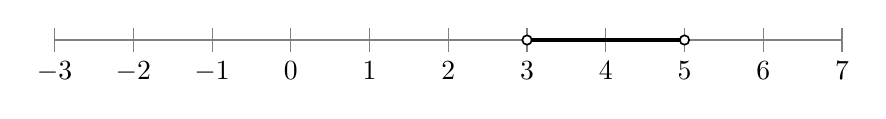
\begin{tikzpicture}[
			  	line/.style = {draw, ultra thick, shorten <=-2pt},
			  	La/.style = {line, shorten >=-2pt,
			  		{Circle[length=4pt, line width=1pt]}-{Circle[length=4pt,line width=1pt, fill=white]}},
			  	Lb/.style = {line, shorten >=-2pt,
			  		{Circle[length=4pt, line width=1pt, fill=white]}-{Circle[length=4pt, line width=1pt]}},
			  	Lc/.style = {line,
			  		{Circle[length=4pt, line width=1pt, fill=white]}-{Triangle[length=4pt, line width=1pt]}},
			  	Lq/.style = {line, shorten >=-2pt,
			  		{Circle[length=4pt, line width=0.6pt, fill=white]}-{Circle[length=4pt,line width=0.6pt, fill=white]}},
			  	Ld/.style = {line, shorten >=-2pt,
			  		{Circle[length=4pt, line width=1pt]}-{Circle[length=4pt, line width=1pt]}},	
			  		]
			  		
			  		\draw[gray] (-3,0) -- (7,0);    % <---
			  		\foreach \i in {-3,-2,...,7} % numbers on line
			  		\draw[gray] (\i,0.15) -- ++ (0,-0.3)    % <---
			  		node[below,text=black] {$\i$}; % tick and their labels
			  		
			  		\draw[Lq] (3,0)--(5,0);
			  	\end{tikzpicture}
		\end{center}
		\item Intervalo Cerrado. \\
		Intervalo cerrado, [a, b], es el conjunto de todos los números reales mayores o iguales que a y menores o iguales que b.
		
		\item[1. ] Forma Intervalo.
		\begin{equation*}
			\left[3,5\right]
		\end{equation*}
		\item[2. ] Forma Conjunto.
		\begin{equation*}
			x : x\in\mathbb{R} / 3 \leq x \leq 5
		\end{equation*}
		\item[3. ] Forma Grafica
		\begin{center}
			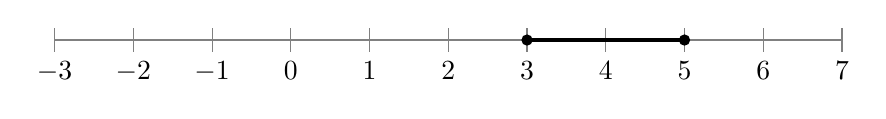
\begin{tikzpicture}[
				line/.style = {draw, ultra thick, shorten <=-2pt},
				La/.style = {line, shorten >=-2pt,
					{Circle[length=4pt, line width=1pt]}-{Circle[length=4pt,line width=1pt, fill=white]}},
				Lb/.style = {line, shorten >=-2pt,
					{Circle[length=4pt, line width=1pt, fill=white]}-{Circle[length=4pt, line width=1pt]}},
				Lc/.style = {line,
					{Circle[length=4pt, line width=1pt, fill=white]}-{Triangle[length=4pt, line width=1pt]}},
				Lq/.style = {line, shorten >=-2pt,
					{Circle[length=4pt, line width=1pt, fill=white]}-{Circle[length=4pt,line width=1pt, fill=white]}},
				Ld/.style = {line, shorten >=-2pt,
					{Circle[length=4pt, line width=1pt]}-{Circle[length=4pt, line width=1pt]}},	
				]
				
				\draw[gray] (-3,0) -- (7,0);    % <---
				\foreach \i in {-3,-2,...,7} % numbers on line
				\draw[gray] (\i,0.15) -- ++ (0,-0.3)    % <---
				node[below,text=black] {$\i$}; % tick and their labels
				
				\draw[Ld] (3,0)--(5,0);
				
			\end{tikzpicture}
		\end{center}
		\item Intervalo semi abierto por izquierda. \\
		Intervalo semiabierto por la izquierda, (a, b], es el conjunto de todos los números reales mayores que a y menores o iguales que b.
		\item[1. ] Forma Intervalo.
		\begin{equation*}
			(3,5]
		\end{equation*}
		\item[2. ] Forma Conjunto.
		 \begin{equation*}
		 	x: x\in\mathbb{R}/3<x\leq5
		 \end{equation*}
		\item[3. ] Forma grafica.
		\begin{center}
			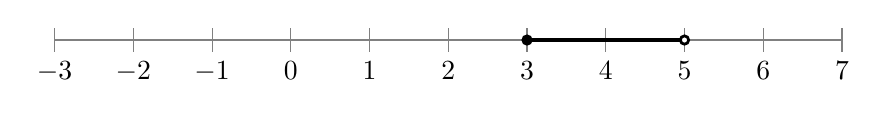
\begin{tikzpicture}[
				line/.style = {draw, ultra thick, shorten <=-2pt},
				La/.style = {line, shorten >=-2pt,
					{Circle[length=4pt, line width=1pt]}-{Circle[length=4pt,line width=1pt, fill=white]}},
				Lb/.style = {line, shorten >=-2pt,
					{Circle[length=4pt, line width=1pt, fill=white]}-{Circle[length=4pt, line width=1pt]}},
				Lc/.style = {line,
					{Circle[length=4pt, line width=1pt, fill=white]}-{Triangle[length=4pt, line width=1pt]}},
				Lq/.style = {line, shorten >=-2pt,
					{Circle[length=4pt, line width=1pt, fill=white]}-{Circle[length=4pt,line width=1pt, fill=white]}},
				Ld/.style = {line, shorten >=-2pt,
					{Circle[length=4pt, line width=1pt]}-{Circle[length=4pt, line width=1pt]}},	
				]
				
				\draw[gray] (-3,0) -- (7,0);    % <---
				\foreach \i in {-3,-2,...,7} % numbers on line
				\draw[gray] (\i,0.15) -- ++ (0,-0.3)    % <---
				node[below,text=black] {$\i$}; % tick and their labels
				
				\draw[La] (3,0) -- (5,0) ;
			\end{tikzpicture}
		\end{center}
		\item Intervalo semi abierto por derecha. \\
		Intervalo semiabierto por la derecha, [a, b), es el conjunto de todos los números reales mayores o iguales que a y menores que b.
		\item[1. ] Forma Intervalo.
		\begin{equation*}
			[3,5)
		\end{equation*}
		\item[2. ] Forma Conjunto.
		\begin{equation*}
			x: x\in\mathbb{R}/3\leq x <5
		\end{equation*}
		\item[3. ] Forma grafica.
		\begin{center}
			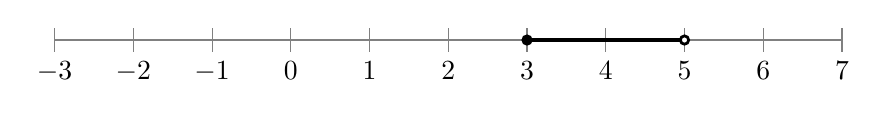
\begin{tikzpicture}[
				line/.style = {draw, ultra thick, shorten <=-2pt},
				La/.style = {line, shorten >=-2pt,
					{Circle[length=4pt, line width=1pt]}-{Circle[length=4pt,line width=1pt, fill=white]}},
				Lb/.style = {line, shorten >=-2pt,
					{Circle[length=4pt, line width=1pt, fill=white]}-{Circle[length=4pt, line width=1pt]}},
				Lc/.style = {line,
					{Circle[length=4pt, line width=1pt, fill=white]}-{Triangle[length=4pt, line width=1pt]}},
				Lq/.style = {line, shorten >=-2pt,
					{Circle[length=4pt, line width=1pt, fill=white]}-{Circle[length=4pt,line width=1pt, fill=white]}},
				Ld/.style = {line, shorten >=-2pt,
					{Circle[length=4pt, line width=1pt]}-{Circle[length=4pt, line width=1pt]}},	
				]
				
				\draw[gray] (-3,0) -- (7,0);    % <---
				\foreach \i in {-3,-2,...,7} % numbers on line
				\draw[gray] (\i,0.15) -- ++ (0,-0.3)    % <---
				node[below,text=black] {$\i$}; % tick and their labels
				
				\draw[La] (3,0) -- (5,0) ;
			\end{tikzpicture}
		\end{center}
	\end{itemize}

	
	
	\section{Pitagóricas en recta real}
	\begin{theo}
		Representar números reales en una recata real con tanta aproximación puede ser a menudo algo muy complejo, pero hay casos que se puede hacer con el famoso teorema de pitagoras, de una forma exacta.
	\end{theo}
	
	Ejemplo de esto: \\
	Representar en una recta real $\sqrt{5}$.
	
\begin{center}
	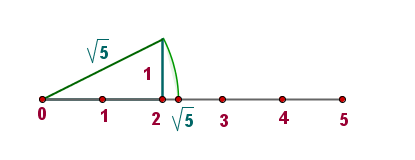
\includegraphics{screenshot001}
\end{center}
	
	
	\begin{itemize}
		\item[1. ]  Tomamos un rectángulo de base 2  y lado 1 . Entonces, usando el teorema de Pitágoras sabemos que su diagonal mide $\sqrt{5}$
		
		\item[2. ] En efecto, Pues $2^2 + 1^2 = d^2$, de donde $5=d^2$, por lo tanto $d=\sqrt{5}$
		
		\item[3. ]Basta agarrar esta medida y transportarla con el compás (tomando centro en 0 y con radio la diagonal de nuestro rectángulo). De este modo, representamos en la recta real el número $\sqrt{5}$
	\end{itemize}
	
	
	 \begin{center}
	 	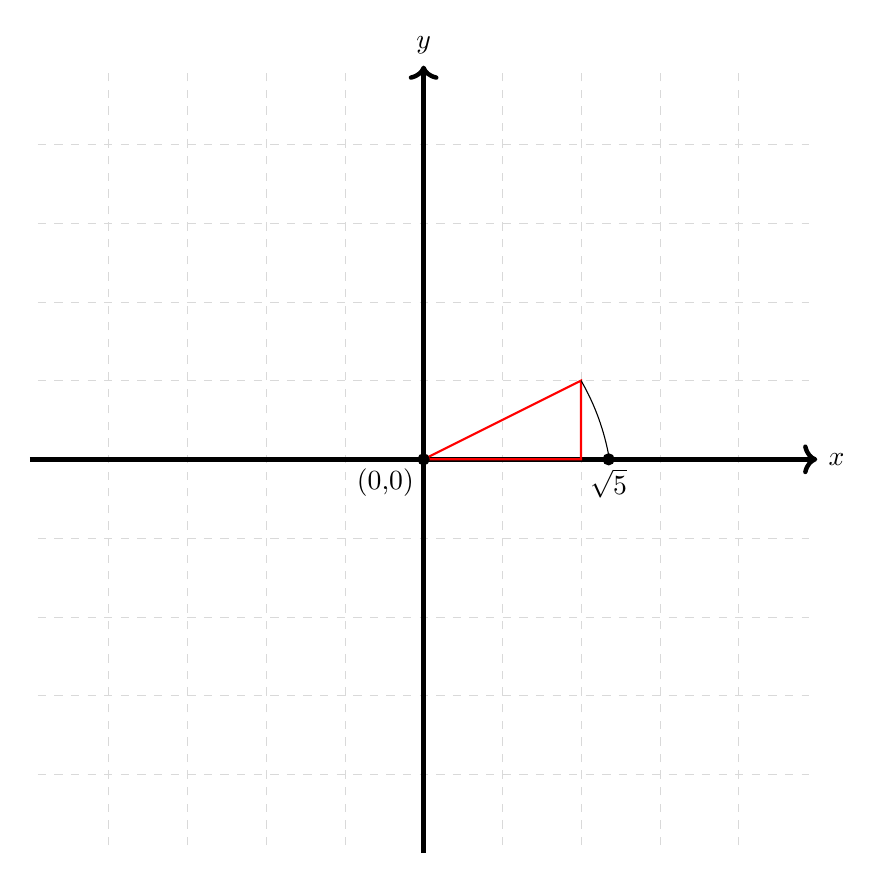
\begin{tikzpicture}
	 		\draw[help lines, color=gray!30, dashed] (-4.9,-4.9) grid (4.9,4.9);
	 		\draw[->,ultra thick] (-5,0)--(5,0) node[right]{$x$};
	 		\draw[->,ultra thick] (0,-5)--(0,5) node[above]{$y$};
	 		\draw[red, thick] (0,0) -- (2,0) -- (2,1) -- cycle ;
	 		\draw (2,1) arc (30:10:3);
	 		\filldraw[black] (0,0) circle (2pt) node[anchor=north east]{(0,0)};
	 		\filldraw[black] (2.35,0) circle (2pt) node[anchor=north] {$\sqrt{5}$};
	 	\end{tikzpicture}
	 \end{center}
	 
	 
	 
	\section{Errores, relativos, porcentuales y absolutos}
	\subsection{Error Relativo}
	
	\subsection{Error Absoluto}
	
	\subsection{Error Porcentual \% }
	
	
	\section{Funciones}
	\subsection{Función Cuadrática}
	
	
	\subsection{Función Modulo}
	
	
	\subsection{Función Polinómica}
	
	
	\subsection{Función Exponencial y Logarítmica}
	
	
	\subsection{Función Homogénea}
	
	
	\section{Números Complejos}
	
	\subsection{Operaciones con números complejos}
	
	\subsection{Operaciones combinadas con números complejos}
	
	
	
	\begin{theo}
		
	\end{theo}
\end{document}